\section*{Actividad}

Considerando la información presentada en las sesiones teóricas de Marzo (incluyendo la disponible en los videos 
recomendados en clase), para cada uno de los siguientes campos vectoriales $ \vec{F}(x,y) $ produzca:

\begin{itemize}
    \item Un desarrollo hecho a mano del cálculo de la divergencia del campo vectorial $ \nabla \cdot \vec{F}(x,y) $ 
    y del rotacional $ \nabla \times \vec{F}(x,y)$
    \item El cálculo manual de la divergencia en tres (3) puntos diferentes del plano $xy$
    \item El cálculo manual del rotacional en los mismos tres (3) puntos del plano usados en el ítem anterior
    \item Una representación visual del campo escalar correspondiente a la divergencia como gráfico de superficie 
    usando \texttt{matplotlib}
    \item Una representación visual del campo vectorial $ \vec{F}(x,y) $ usando también \texttt{matplotlib} 
    (por ejemplo usando \texttt{pyplot.quiver})
\end{itemize}
    

\section*{Solución}

\subsection{Contexto y Teoría}

Como ya habíamos visto en las sesiones teóricas, la divergencia y el rotacional son dos conceptos 
fundamentales en el análisis de campos vectoriales. La divergencia mide la tasa de cambio neta de un campo vectorial en 
un punto, mientras que el rotacional mide la tendencia de un campo a rotar alrededor de un punto dado.

Pero que matemáticamente como definiriamos la divergencia y el rotacional?

\subsection{Operador Nabla $\nabla$}
El operador nabla, denotado por $\nabla$, es un operador vectorial que se utiliza para calcular la divergencia y el 
rotacional de un campo vectorial. En coordenadas cartesianas, el operador nabla se puede definir en $R^3$ como:
$$
\nabla = \left( \frac{\partial}{\partial x}, \frac{\partial}{\partial y}, \frac{\partial}{\partial z} \right)
$$
puede parecer un poco incomodo verlo de la manera anterior, debido a que no tiene mucho sentido entender que haya 
derivadas parciales sin nada dentro de un vector, por lo que matemáticamente no es muy estricata esta manera, pero 
resulta favorable para poder trabajar con el operador y definirlo en los siguientes operadores.
\subsubsection{Divergencia}
La  divergencia de un campo vectorial se puede definir como el producto punto entre dos vectores, el operador nabla y el
campo vectorial $$ \nabla \cdot \vec{F} = 
\left( \frac{\partial}{\partial x}, \frac{\partial}{\partial y}, \frac{\partial}{\partial z} \right) 
\cdot \left( P, Q, R \right) $$
donde $P$, $Q$ y $R$ son las componentes del campo vectorial $\vec{F}$. Al realizar el producto punto, obtenemos: 
$$ 
\nabla \cdot \vec{F} = \frac{\partial P}{\partial x} + \frac{\partial Q}{\partial y} + \frac{\partial R}{\partial z}
$$
La divergencia es util en varios contextos ya que nos puede ayudar a conocer el comportamiento en distintos puntos
de un campo vectorial, por ejemplo, si la divergencia de un campo resulta positiva, tenemos que concluir que la cantidad
de flujo que entra es menor a la cantidad de flujo que sale, se puede ver como una fuente, mientras que si la divergencia
es menor que 0, tenemos que la cantidad que entra es mayor que la cantidad que sale, siendo un sumidero el ejemplo
perfecto, pero si la divergencia de un campo resulta en 0, entonces concluimos que entra la misma cantidad que sale, 
por lo que se dice que el campo es incompresible, ya que no hay fuentes ni sumideros.

Algo que también podemos resaltar y concretar de la divergencia es que nos sirve para varios teoremas importantes en el 
cálculo vectorial, como el teorema de Gauss, que nos dice que el flujo de un campo vectorial a través de una superficie
cerrada es igual a la integral de la divergencia del campo vectorial sobre el volumen encerrado por la superficie. Lo que
se expresa de la siguiente manera:
$$ \oiint_S \vec{F} \cdot d\vec{S} = \iiint_V (\nabla \cdot \vec{F}) \, dV $$

Otro uso util es que la divergencia también se puede ver en ecuaciones armonicas, por ejemplo para conocer si una función
escalar $f(x,y)$ es la función potencial de un campo electrostático, es necesario que el operador \textbf{Laplaciano}
de nuestra función escalar sea igual a 0, pero quien es el \textbf{Laplaciano}? el operador Laplaciano se define como
la divergencia del  gradiente de una función escalar, es decir, $ \nabla^2 f = \nabla \cdot (\nabla f) $ en algunos libros
se puede ver como  $ \Delta f $.
\subsubsection{Rotacional}
El rotacional de un campo vectorial se puede definir como el producto cruz entre el operador nabla y el campo vectorial 
$$ \nabla \times \vec{F} = 
\ \left( \frac{\partial}{\partial x}, \frac{\partial}{\partial y}, \frac{\partial}{\partial z} \right) 
\times \left( P, Q, R \right) $$
Al realizar el producto cruz, obtenemos:
$$
\nabla \times \vec{F} = \left( \frac{\partial R}{\partial y} - \frac{\partial Q}{\partial z}, \frac{\partial P}{\partial z} 
- \frac{\partial R}{\partial x}, \frac{\partial Q}{\partial x} - \frac{\partial P}{\partial y} \right)$$

El rotacional es útil para conocer la tendencia de un campo a rotar alrededor de un punto dado, por ejemplo, 
si el rotacional es positivo, entonces el campo tiende a rotar en sentido antihorario, si es negativo, rota en sentido horario,
y si es 0 significa que no tiene rotación al rededor del punto, el rotacional es más complicado de calcular en estos casos
para ello es util utilizar el metodo de coofactores, que es un método que sirve para calcular el producto cruz entre dos vectores
como si se estuviera calculando el determinante de una matriz 3x3, es decir que lo podríamos escribir de la siguiente manera:
$$ \nabla \times \vec{F} =
\begin{vmatrix}
\hat{i} & \hat{j} & \hat{k} \\
\frac{\partial}{\partial x} & \frac{\partial}{\partial y} & \frac{\partial}{\partial z} \\
P & Q & R
\end{vmatrix} $$
donde $\hat{i}$, $\hat{j}$ y $\hat{k}$ son los vectores unitarios en las direcciones $x$, $y$ y $z$ respectivamente.
hagamos un ejemplo general donde calculamos el rotacional de un campo vectorial $ \vec{F} = \left( P, Q, 0 \right) \quad
\text{donde} \ P, Q \text{ son funciones de } x \text{ y } y $
esto nos servira para los ejemplos que veremos más adelante donde calcularemos  el  rotacional de campos vectoriales 
en el plano $$ \nabla \times \vec{F} =
\begin{vmatrix}
\hat{i} & \hat{j} & \hat{k} \\
\frac{\partial}{\partial x} & \frac{\partial}{\partial y} & \frac{\partial}{\partial z} \\
P & Q & 0
\end{vmatrix} = \hat{i}\left(\frac{\partial R}{\partial y} - \frac{\partial Q}{\partial z}\right) + \hat{j}
\left(\frac{\partial P}{\partial z} - \frac{\partial 0}{\partial x}\right) + \hat{k}\left(\frac{\partial Q}{\partial x} 
- \frac{\partial P}{\partial y}\right)$$ como P y Q no dependen de z, entonces las derivadas parciales con respecto a z 
son 0, por lo que el rotacional se reduce a: $$ \nabla \times \vec{F} = \hat{k}\left(\frac{\partial Q}{\partial x} - 
\frac{\partial P}{\partial y}\right) $$
esto que acabamos de hacer como un pequeño repaso de cálculo vectorial no solo es util para calcular el rotacional sino
también para utilizar un teorema importante en el cálculo vectorial, el teorema de Green 
(este utiliza el rotacional solo en su componente z) y el teorema de Stokes, una forma 
de verlo es que el teorema de Green es una versión en 2 dimensiónes del teorema de Stokes (mirelo como si Stokes fuera
el padre de Green), los teoremas nos sirven hacer cambios entre integrales de línea, integrales de superficie e integrales 
de volumen. aquí si me extiendo demasiado, pero pues es interesante para el repaso.

Otra cosa relevante del rotacional es que nos sirve para conocer si un campo vectorial es conservativo o no, aunque necesita
una condición adicional, que el dominio del campo  vectorial sea simplemente conexo, pero si esto se cumple y el rotacional
es igual a 0 podemos decir que el campo vectorial es conservativo, significa que para el campo vectorial podemos encontrar
una función potencial, una función que cuando apliquemos el rotacional, nos devuelve el campo vectorial original.
Además de ser util cuando calculamos integrales de línea que comienzan y termian en el mismo punto, ya que si el campo vectorial
es conservativo, la integral de línea \textbf{SIEMPRE} sera igual a 0, sin importar la ruta que se tome, este mismo concepto
se aplica si calculamos una integral de línea entre dos puntos diferentes y dos rutas distintas, si es conservativo
ambas rutas daran el mismo resultado, es util cuando se trata con curvas muy complejas.

Por ultimo podemos resaltar que si la componente R es igual a 0 como habíamos dicho obtenemos una función vectorial 
que solo tiene componenten en el eje z, esto util ya que en realidad estamos tratando con una función escalar,
viendo de la siguiente manera $$ \nabla \times \vec{F} = \hat{k}\left(\frac{\partial Q}{\partial x} - 
\frac{\partial P}{\partial y}\right) \text{donde} z = \frac{\partial Q}{\partial x} - \frac{partial P}{\partial y}$$

Otra forma que utilice para desarrollar el rotacional y gráficarlo en matplotlib fue visualizarlo como un mapa de calor, 
es decir, que cada punto del plano xy tenga un color diferente dependiendo del valor del rotacional en ese punto. Relacionando
como habíamos mencionado el significado que se le da dependiendo del valor del rotacional.
en general el libro de openstax \cite{openstax_divergencia_rizo} tiene la sección 6.5 \textbf(Divergencia y Rizo) aunque 
la verdad no sé porque lo traducen como rizo, pero es la más detallada sobre la divergencia y el rotacional, con aplicaciones
a la física y a la ingeniería sin tanta teoría, lo utilice para esta parte a diferencia de la actividad de gradientes que
utilice en su mayoría el marsden tromba \cite{marsden_tromba_calculo_vectorial}

\section{Solución A Mano y evaluación de 3 puntos}

\begin{figure}[H]
\centering
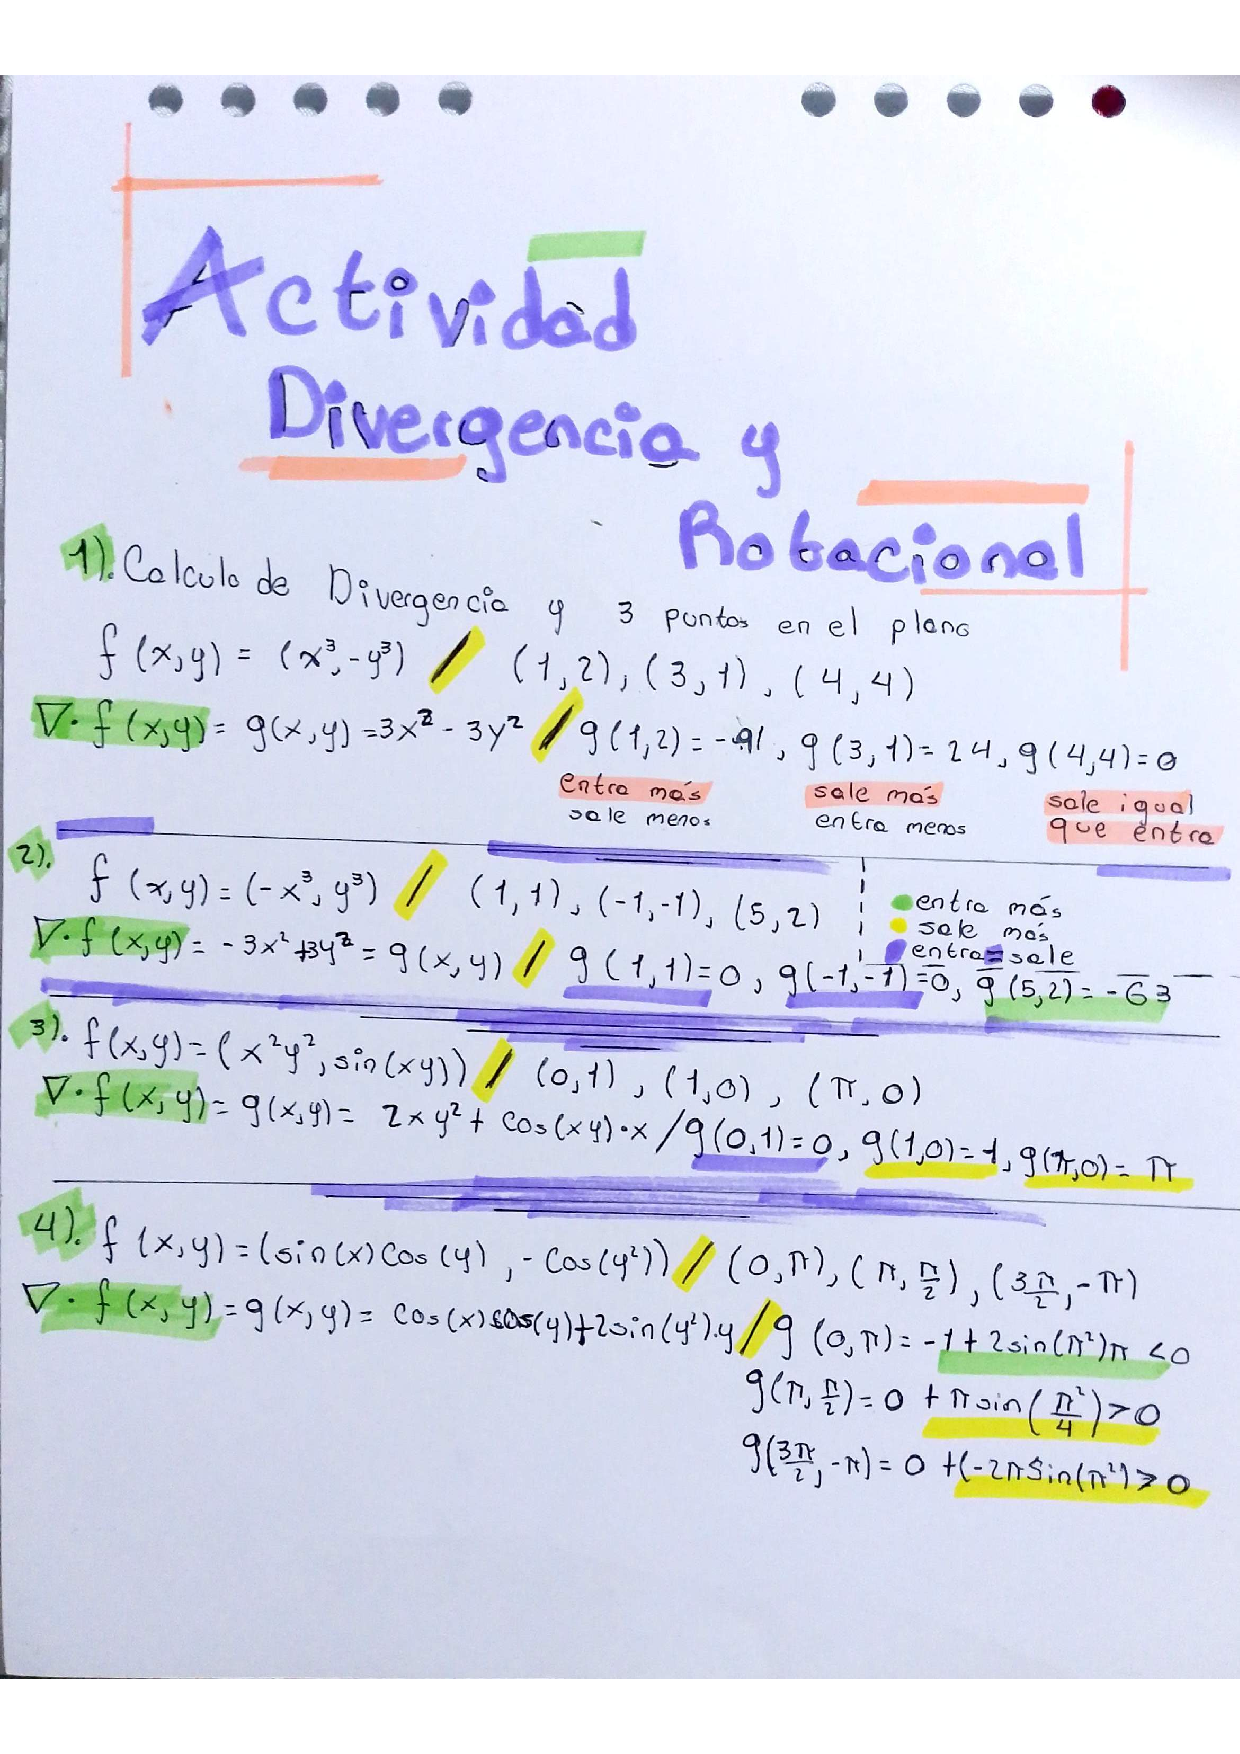
\includegraphics[width=\linewidth,page=1]{Images/Div_Rot.pdf}
\caption{Desarrollo manual del cálculo de la divergencia (parte 1).}
\end{figure}

\begin{figure}[H]
\centering
\includegraphics[width=\linewidth,page=2]{Images/Div_Rot.pdf}
\caption{Desarrollo manual del cálculo de la divergencia y el rotacional (parte 2).}
\end{figure}

\begin{figure}[H]
\centering
\includegraphics[width=\linewidth,page=3]{Images/Div_Rot.pdf}
\caption{Desarrollo manual del cálculo del rotacional (parte 3).}
\end{figure}

\section{Código Python y Gráficas}

Las siguientes visualizaciones fueron generadas utilizando Python y la biblioteca \texttt{matplotlib}.
\begin{lstlisting}[language=Python]
import numpy as np
import matplotlib.pyplot as plt
from mpl_toolkits import mplot3d
\end{lstlisting}
Los campos vectoriales de la actividad y los puntos escogidos son los siguientes:
\subsection{ Campos Vectoriales a trabajar y sus puntos}
\begin{enumerate}
    \item $ f(x,y) = \left(x^3,-y^3\right) \quad \left(1,2\right) \quad \left(3,1\right) \quad \left(4,4\right)$
    \item $ f(x,y) = \left(-x^3,y^3\right)\quad \left(1,1\right) \quad \left(-1,-1\right) \quad \left(5,2\right) $
    \item $ f(x,y) = \left( x^2y^2,\sin(xy)\right) \quad \left(0,1\right) \quad \left(1,0\right) \quad \left(\pi ,0\right) $
    \item $ f(x,y) = \left( \sin(x)\cos(y),-cos(y^2)\right) \quad \left(0,\pi\right) \quad \left(\pi,\dfrac{\pi}{2}\right) \quad \left(\dfrac{3\pi}{2} ,-\pi\right)$
    \item $ f(x,y) = \left(x^3+4x^2y, -5xy^2-y^3\right) \quad \left(0,1\right) \quad \left(1,2\right) \quad \left(1,-1\right) $
    \item $ f(x,y) = \left(\cos(x^3) + 4\sin(x^2)\cos(y), -5x^2y^3+2x^3y^2\right) \quad \left(0,0\right) \quad \left(\pi,0\right) \quad \left(0,\pi\right) $
\end{enumerate}

\subsection{Divergencias}
\begin{enumerate}
    \item $ \nabla \cdot f(x,y) = 3x^2 - 3y^2 $
    \item $ \nabla \cdot f(x,y) = -3x^2 + 3y^2 $
    \item $ \nabla \cdot f(x,y) = 2xy^2 + x^2y\cos(xy) $
    \item $ \nabla \cdot f(x,y) = -\sin(x)\sin(y) $
    \item $ \nabla \cdot f(x,y) = 3x^2 + 8xy - 5y^2 $
    \item $ \nabla \cdot f(x,y) = -3x^2\sin(x^3) + 8x\cos(x^2)\cos(y) - 15x^2y^2 + 4x^3y $
\end{enumerate}

\begin{lstlisting}[language=Python]
# 1. Definimos los ejes (vectores 1D)
range_val = np.linspace(-20, 20, 50)

# 2. CREAMOS LA MALLA
x = np.outer(np.linspace(-3, 3, 100), np.ones(100))
y = x.copy().T
# 3. Calculamos Z usando las matrices
z = 3 * x**2 - 3 * y**2

# 4. Graficamos (usando una proyeccion 3D)
fig, ax = plt.figure(figsize=(10, 8)), plt.axes(projection='3d') # Importante definir que es 3D
ax.plot_surface(x, y, z, cmap='inferno')
ax.view_init(elev=45, azim=45)
ax.set_title(r"1. $\nabla \cdot f(x,y) = 3x^2-3y^2$", fontsize=16, color='navy', pad=20)
fig.savefig('Images/Ejercicio_1_Divergencia.png', dpi=150, bbox_inches='tight')
plt.show()
\end{lstlisting}
\begin{figure}[H]
\centering
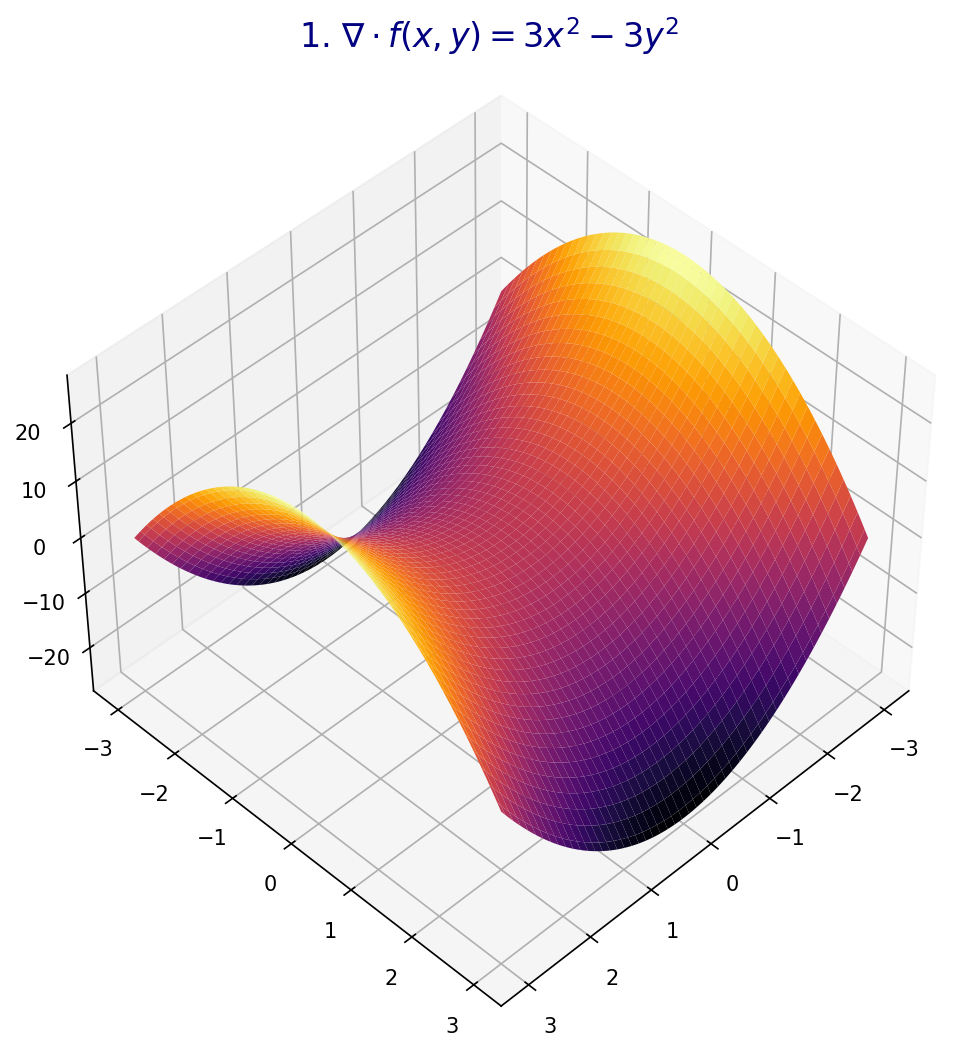
\includegraphics[width=0.8\linewidth]{Images/Ejercicio_1_Divergencia.png}
\caption{Gráfico de superficie de la divergencia del campo vectorial $f(x,y) = \left(x^3,-y^3\right)$.}
\end{figure}

\begin{lstlisting}[language=Python]
# 1. Definimos los ejes (vectores 1D)
range_val = np.linspace(-20, 20, 50)

# 2. CREAMOS LA MALLA
x = np.outer(np.linspace(-3, 3, 100), np.ones(100))
y = x.copy().T
# 3. Calculamos Z usando las matrices
z = -3 * x**2 + 3 * y**2

# 4. Graficamos (usando una proyeccion 3D)
fig, ax = plt.figure(figsize=(10, 8)), plt.axes(projection='3d') # Importante definir que es 3D
ax.plot_surface(x, y, z, cmap='inferno')
ax.view_init(elev=45, azim=45)
ax.set_title(r"2. $\nabla \cdot f(x,y) = 3y^2-3x^2$", fontsize=16, color='navy', pad=20)
fig.savefig('Images/Ejercicio_2_Divergencia.png', dpi=150, bbox_inches='tight')
plt.show()
\end{lstlisting}
\begin{figure}[H]
\centering
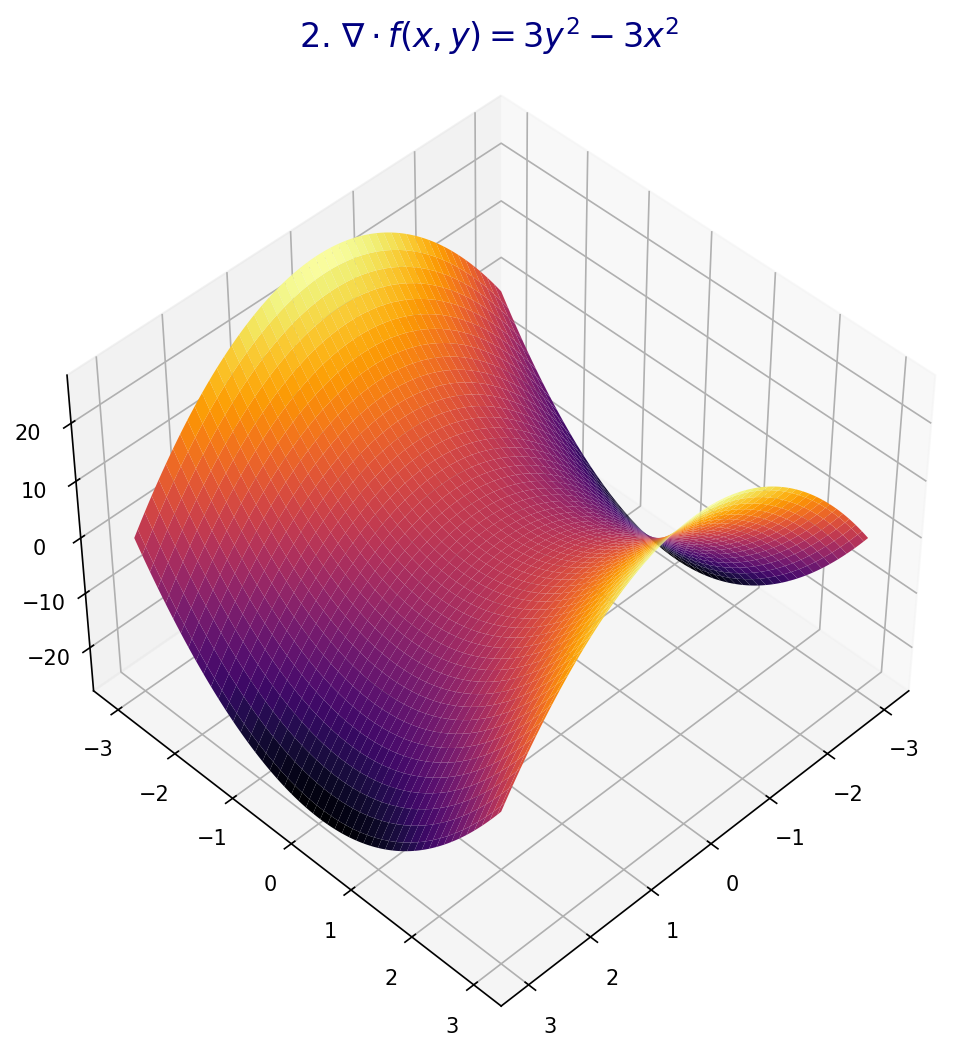
\includegraphics[width=0.8\linewidth]{Images/Ejercicio_2_Divergencia.png}
\caption{Gráfico de superficie de la divergencia del campo vectorial $f(x,y) = \left(-x^3,y^3\right)$.}
\end{figure}

\begin{lstlisting}[language=Python]
# 1. Definimos los ejes (vectores 1D)
range_val = np.linspace(-20, 20, 50)

# 2. CREAMOS LA MALLA
x = np.outer(np.linspace(-3, 3, 100), np.ones(100))
y = x.copy().T
# 3. Calculamos Z usando las matrices
z = 2 * x * y**2 + np.cos(x * y) * x

# 4. Graficamos (usando una proyeccion 3D)
fig, ax = plt.figure(figsize=(10, 8)), plt.axes(projection='3d') # Importante definir que es 3D
ax.plot_surface(x, y, z, cmap='inferno')
ax.view_init(elev=45, azim=135)
ax.set_title(r"3. $\nabla \cdot f(x,y) = 2xy^2+cos(xy)x$", fontsize=16, color='navy', pad=20)
fig.savefig('Images/Ejercicio_3_Divergencia.png', dpi=150, bbox_inches='tight')
plt.show()
\end{lstlisting}
\begin{figure}[H]
\centering
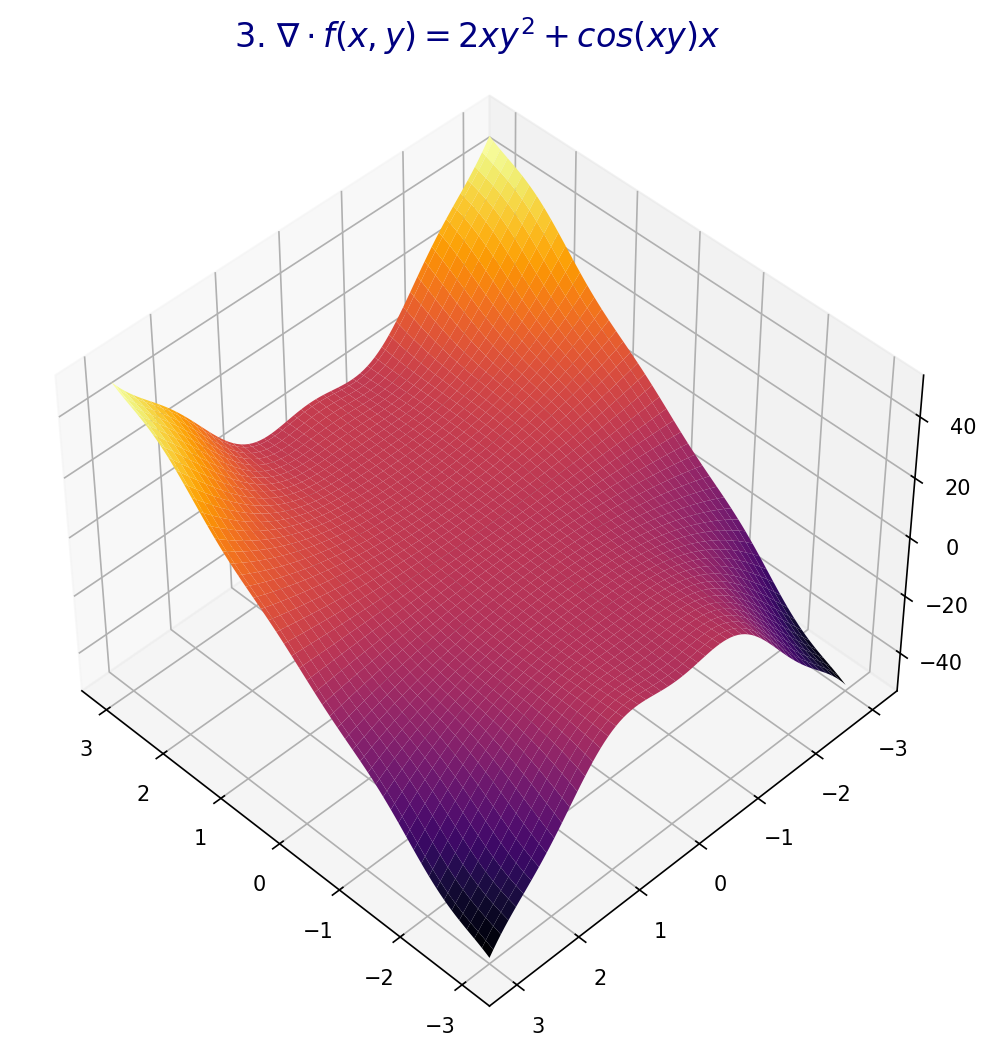
\includegraphics[width=0.8\linewidth]{Images/Ejercicio_3_Divergencia.png}
\caption{Gráfico de superficie de la divergencia del campo vectorial $f(x,y) = \left( x^2y^2,\sin(xy)\right)$.}
\end{figure}    
\begin{lstlisting}[language=Python]
# 1. Definimos los ejes (vectores 1D)
range_val = np.linspace(-20, 20, 50)

# 2. CREAMOS LA MALLA
x = np.outer(np.linspace(-10, 10, 500), np.ones(500))
y = x.copy().T

# 3. Calculamos Z usando las matrices
z = np.cos(x) * np.cos(y) + 2 * y * np.sin(y**2)
# 4. Graficamos (usando una proyeccion 3D)
fig = plt.figure(figsize=(10, 8))
ax = plt.axes(projection='3d') # Importante definir que es 3D

ax.plot_surface(x, y, z, cmap='inferno')
ax.view_init(elev=60, azim=45)
 
ax.set_title(r"4. $\nabla \cdot f(x,y) = \cos(x)\cos(y) + 2y\sin(y^2)$", fontsize=16, color='navy', pad=20)
fig.savefig('Images/Ejercicio_4_Divergencia.png', dpi=150, bbox_inches='tight')

plt.show()
\end{lstlisting}
\begin{figure}[H]
\centering
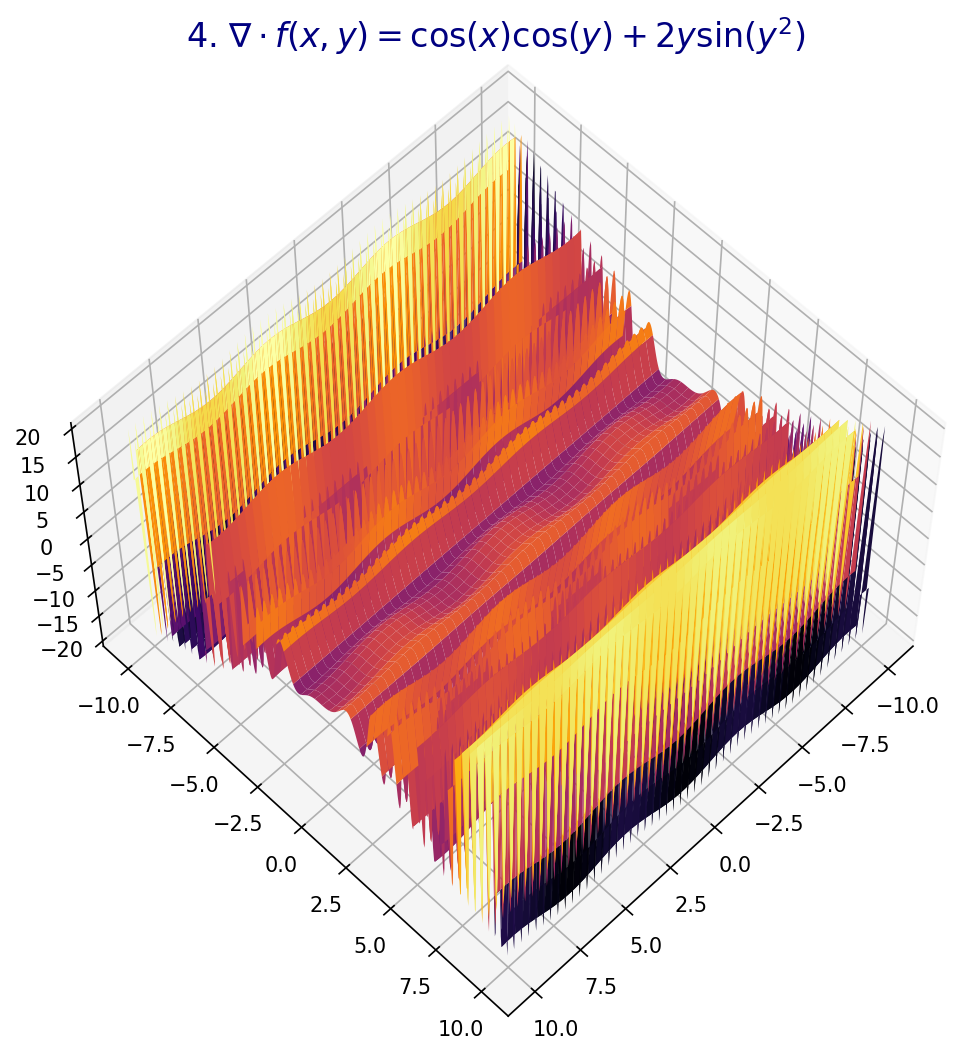
\includegraphics[width=0.8\linewidth]{Images/Ejercicio_4_Divergencia.png}
\caption{Gráfico de superficie de la divergencia del campo vectorial $f(x,y) = \left( \sin(x)\cos(y),-cos(y^2)\right)$.}
\end{figure}


\begin{lstlisting}[language=Python]
# 1. Definimos los ejes (vectores 1D)
range_val = np.linspace(-20, 20, 50)

# 2. CREAMOS LA MALLA
x = np.outer(np.linspace(-5, 5, 50), np.ones(50))
y = x.copy().T

# 3. Calculamos Z usando las matrices
z = 3 * x**2 - 2 * x * y - 3 * y**2
# 4. Graficamos (usando una proyeccion 3D)
fig = plt.figure(figsize=(10, 8))
ax = plt.axes(projection='3d') # Importante definir que es 3D
ax.plot_surface(x, y, z, cmap='inferno')
ax.set_title(r"5. $\nabla \cdot f(x,y) = 3x^2 - 2xy - 3y^2$", fontsize=16, color='navy', pad=20)
fig.savefig('Images/Ejercicio_5_Divergencia.png', dpi=150, bbox_inches='tight')

plt.show()
    
\end{lstlisting}
\begin{figure}[H]
\centering
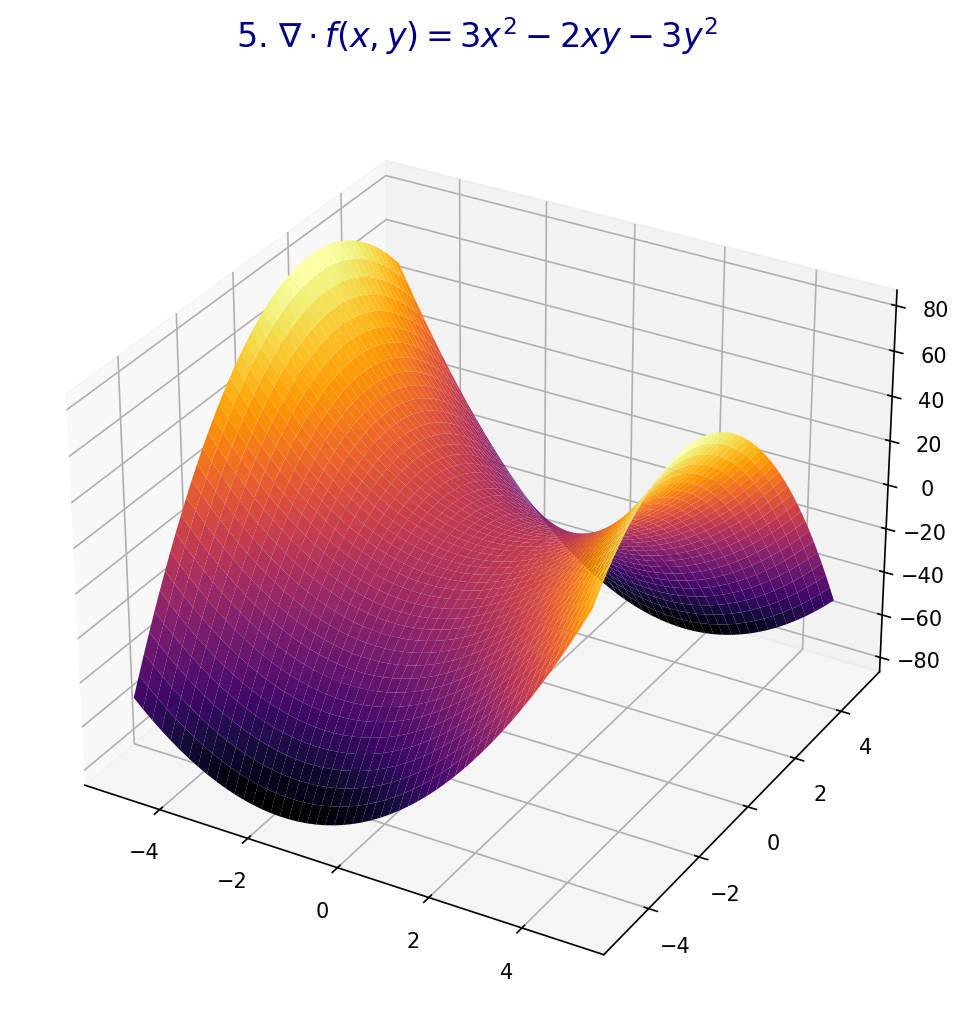
\includegraphics[width=0.8\linewidth]{Images/Ejercicio_5_Divergencia.png}
\caption{Gráfico de superficie de la divergencia del campo vectorial $f(x,y) = \left(x^3+4x^2y, -5xy^2-y^3\right)$.}
\end{figure}

\begin{lstlisting}[language=Python]
# 1. Definimos los ejes (vectores 1D)
range_val = np.linspace(-20, 20, 50)

# 2. CREAMOS LA MALLA
# X e Y ahora son matrices de 50x50
x = np.outer(np.linspace(-1, 1, 1000), np.ones(1000))
y = x.copy().T

# 3. Calculamos Z usando las matrices
z = -3 * x**2 * np.sin(x**3) + 8 * x * np.cos(x**2) * np.cos(y) - 15 * x**2 * y**2 + 4 * x**3 * y
# 4. Graficamos (usando una proyeccion 3D)
fig, ax = plt.figure(figsize=(10, 8)), plt.axes(projection='3d') # Importante definir que es 3D


ax.plot_surface(x, y, z, cmap='inferno')
ax.view_init(elev=60, azim=45)

ax.set_title(r"6. $\nabla \cdot f(x,y) = -3x^2\sin(x^3) + 8x\cos(x^2)\cos(y) - 15x^2y^2 + 4x^3y$", fontsize=16, color='navy', pad=20)
fig.savefig('Images/Ejercicio_6_Divergencia.png', dpi=150, bbox_inches='tight')

plt.show()
\end{lstlisting}
\begin{figure}[H]
\centering
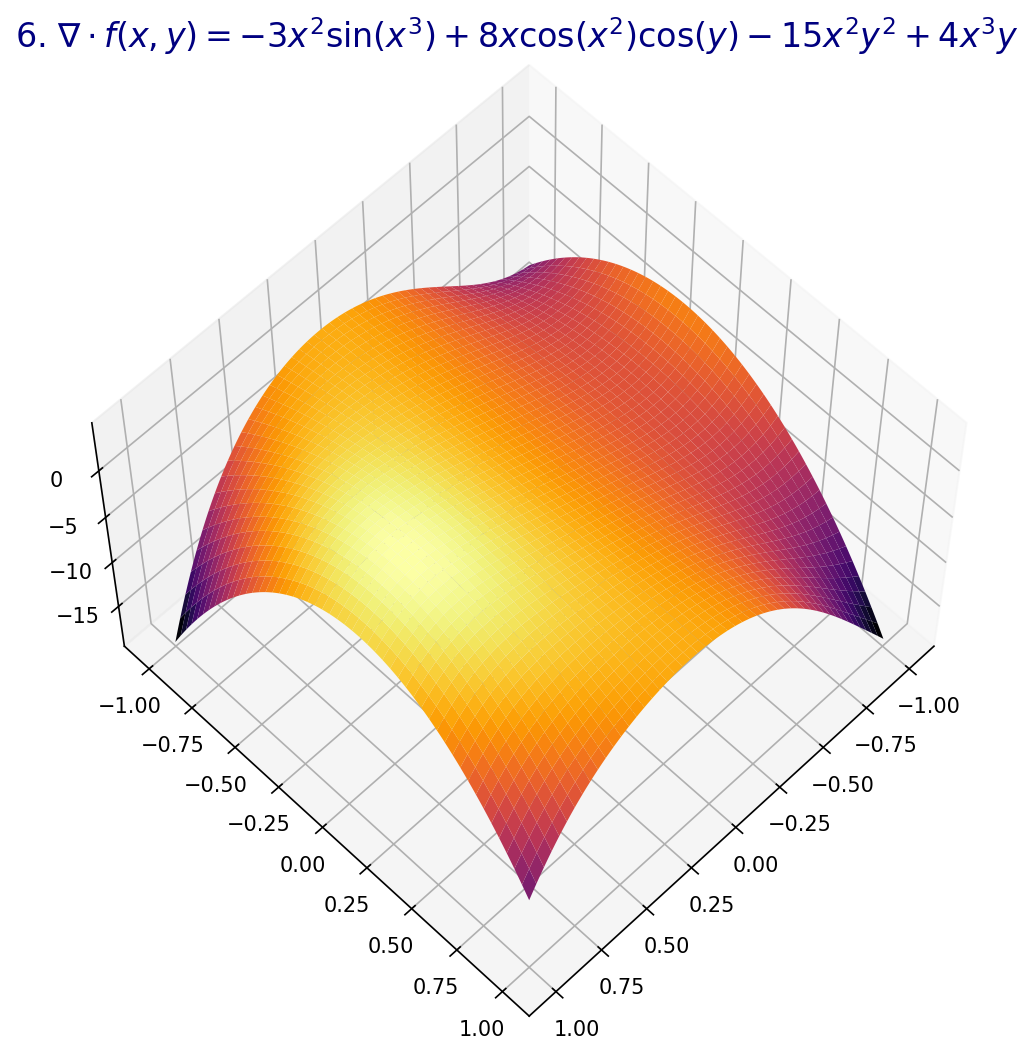
\includegraphics[width=0.8\linewidth]{Images/Ejercicio_6_Divergencia.png}
\caption{Gráfico de superficie de la divergencia del campo vectorial $f(x,y) = \left(\cos(x^3) + 4\sin(x^2)\cos(y), -5x^2y^3+2x^3y^2\right)$.}
\end{figure}

\subsection{Rotacionales}
Por obvias razones, los rotacionales de los campos vectoriales que resultan en el vector 0, no los voy a gráficar,
ya que no tienen rotación y por lo tanto no tienen sentido visualizarlos, hay que tener en cuenta que se verían solo 
como un plano. También se gráfica de dos maneras, visto como un campo escalar $ z = f(x,y) $ y como un mapa de calor, 
donde cada punto del plano xy tiene un color diferente dependiendo del valor del rotacional en ese punto.

\begin{enumerate}
    \item $ \nabla \times f(x,y) = (0,0,0) $
    \item $ \nabla \times f(x,y) = (0,0,0) $
    \item $ \nabla \times f(x,y) = \left(0,0,y\cos(xy) - 2x^2y\right) $
    \item $ \nabla \times f(x,y) = \left(0,0,\sin(x)\sin(y)\right) $
    \item $ \nabla \times f(x,y) = \left(0,0,-5y^2 - 4x^2\right) $
    \item $ \nabla \times f(x,y) = \left(0,0,4\sin(x^2)\sin(y) -10xy^3 +6x^2y^2\right) $
\end{enumerate}

\begin{lstlisting}[language=Python]
# dominio
x = np.linspace(-3,3,200)
y = np.linspace(-3,3,200)

X,Y = np.meshgrid(x,y)

# rotacional
Z = Y*np.cos(X*Y) - 2*X**2*Y

# figura con 2 paneles
fig = plt.figure(figsize=(14,6))

# --- superficie 3D ---
ax1 = fig.add_subplot(1,2,1, projection='3d')

surf = ax1.plot_surface(
    X,Y,Z,
    cmap='inferno',
    edgecolor='none',
    alpha=0.95
)

ax1.view_init(elev=55, azim=35)

ax1.set_title(
r"$z = y\cos(xy) - 2x^2y$",
fontsize=13,
color='navy',
pad=10
)

ax1.set_xlabel("x")
ax1.set_ylabel("y")
ax1.set_zlabel("rotacional")

# --- mapa de temperatura ---
ax2 = fig.add_subplot(1,2,2)

cont = ax2.contourf(
    X,Y,Z,
    levels=40,
    cmap='inferno'
)

ax2.set_title(
r"$\nabla \times F(x,y)$",
fontsize=13,
color='navy'
)

ax2.set_xlabel("x")
ax2.set_ylabel("y")

fig.colorbar(
    cont,
    ax=ax2,
    label="rotacional"
)

plt.suptitle(
r"3. Rotacional $\nabla \times F(x,y)$",
fontsize=16,
color='darkred'
)

plt.tight_layout()

fig.savefig(
'Imagenes/Ejercicio_3_rotacional.png',
dpi=150,
bbox_inches='tight'
)

plt.show()
\end{lstlisting}
\begin{figure}[H]
\centering
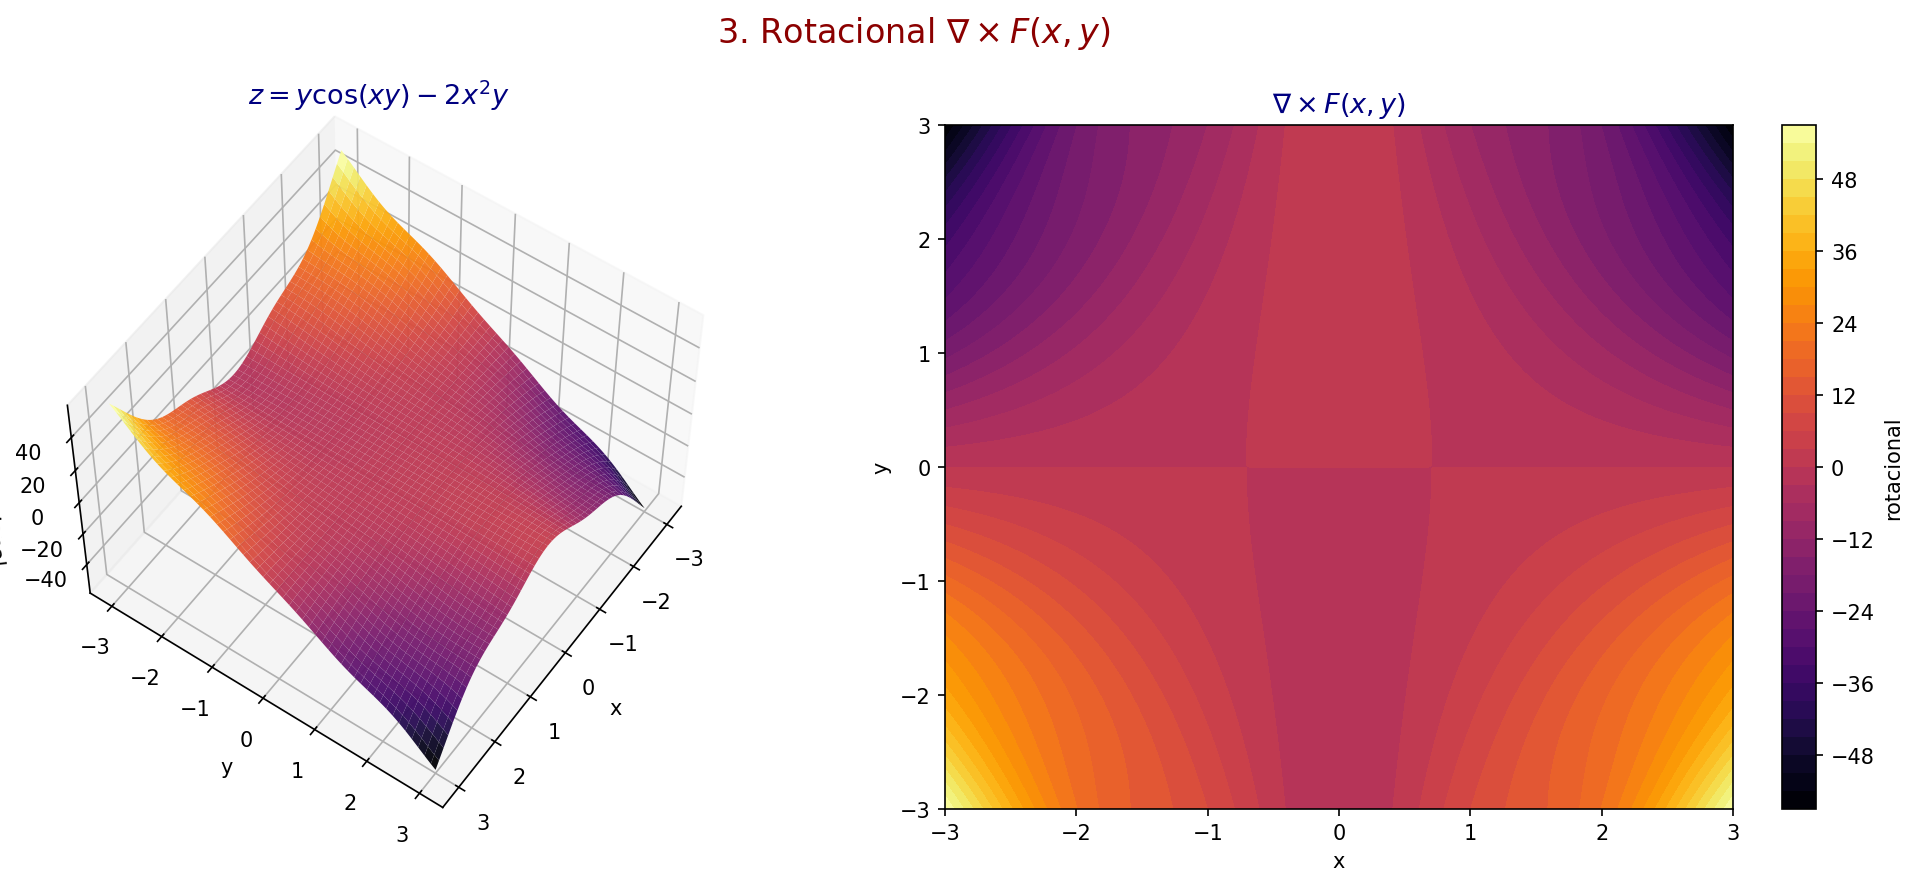
\includegraphics[width=\linewidth]{Images/Ejercicio_3_rotacional.png}
\caption{Gráficos del rotacional del campo vectorial $f(x,y) = \left( x^2y^2,\sin(xy)\right)$ visto como un campo escalar (izquierda) y como un mapa de calor (derecha).}
\end{figure}

\begin{lstlisting}[language=Python]
# dominio
x = np.linspace(-6,6,300)
y = np.linspace(-6,6,300)

X,Y = np.meshgrid(x,y)

# rotacional
Z = np.sin(X)*np.sin(Y)

# figura
fig = plt.figure(figsize=(14,6))

# --- superficie 3D ---
ax1 = fig.add_subplot(1,2,1, projection='3d')

surf = ax1.plot_surface(
    X,Y,Z,
    cmap='inferno',
    edgecolor='none',
    alpha=0.95
)

ax1.view_init(elev=55, azim=35)

ax1.set_title(
r"$z = \sin(x)\sin(y)$",
fontsize=13,
color='navy'
)

ax1.set_xlabel("x")
ax1.set_ylabel("y")
ax1.set_zlabel("rotacional")

# --- mapa de temperatura ---
ax2 = fig.add_subplot(1,2,2)

cont = ax2.contourf(
    X,Y,Z,
    levels=40,
    cmap='inferno'
)

ax2.contour(
    X,Y,Z,
    levels=[0],
    colors='black',
    linewidths=1.2
)

ax2.set_title(
r"$\nabla \times F(x,y)$",
fontsize=13,
color='navy'
)

ax2.set_xlabel("x")
ax2.set_ylabel("y")

fig.colorbar(cont, ax=ax2, label="rotacional")

plt.suptitle(
r"4. Rotacional $\nabla \times F(x,y)$",
fontsize=16,
color='darkred'
)

plt.tight_layout()

fig.savefig(
'Imagenes/Ejercicio_4_rotacional.png',
dpi=150,
bbox_inches='tight'
)

plt.show()
\end{lstlisting}
\begin{figure}[H]
\centering
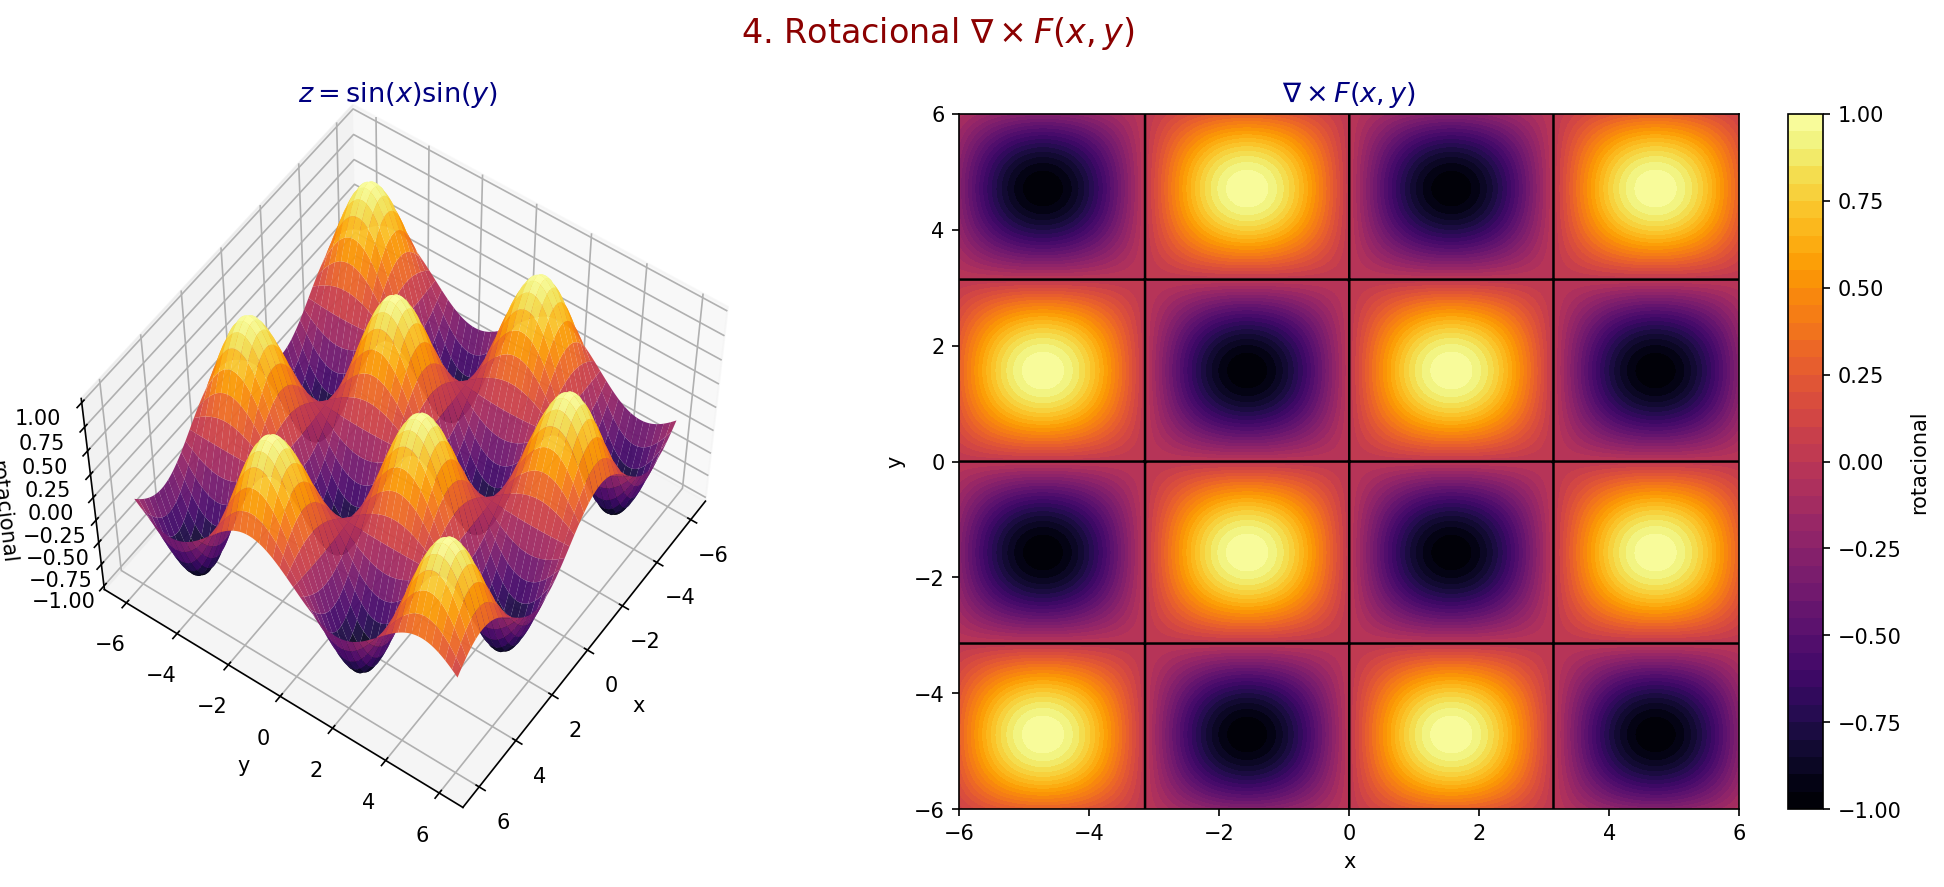
\includegraphics[width=\linewidth]{Images/Ejercicio_4_rotacional.png}
\caption{Gráficos del rotacional del campo vectorial $f(x,y) = \left( \sin(x)\cos(y),-cos(y^2)\right)$ visto como un campo escalar (izquierda) y como un mapa de calor (derecha).}
\end{figure}    

\begin{lstlisting}[language=Python]
# dominio
x = np.linspace(-5,5,300)
y = np.linspace(-5,5,300)

X,Y = np.meshgrid(x,y)

# rotacional
Z = -5*Y**2 - 4*X**2

# figura
fig = plt.figure(figsize=(14,6))

# --- superficie 3D ---
ax1 = fig.add_subplot(1,2,1, projection='3d')

surf = ax1.plot_surface(
    X,Y,Z,
    cmap='inferno',
    edgecolor='none',
    alpha=0.95
)

ax1.view_init(elev=45, azim=35)

ax1.set_title(
r"$z = -5y^2 - 4x^2$",
fontsize=13,
color='navy'
)

ax1.set_xlabel("x")
ax1.set_ylabel("y")
ax1.set_zlabel("rotacional")

# --- mapa de temperatura ---
ax2 = fig.add_subplot(1,2,2)

cont = ax2.contourf(
    X,Y,Z,
    levels=40,
    cmap='inferno'
)

ax2.contour(
    X,Y,Z,
    levels=[0],
    colors='black',
    linewidths=1.2
)

ax2.set_title(
r"$\nabla \times F(x,y)$",
fontsize=13,
color='navy'
)

ax2.set_xlabel("x")
ax2.set_ylabel("y")

fig.colorbar(cont, ax=ax2, label="rotacional")

plt.suptitle(
r"5. Rotacional $\nabla \times F(x,y)$",
fontsize=16,
color='darkred'
)

plt.tight_layout()

fig.savefig(
'Imagenes/Ejercicio_5_rotacional.png',
dpi=150,
bbox_inches='tight'
)

plt.show()
\end{lstlisting}
\begin{figure}[H]
\centering
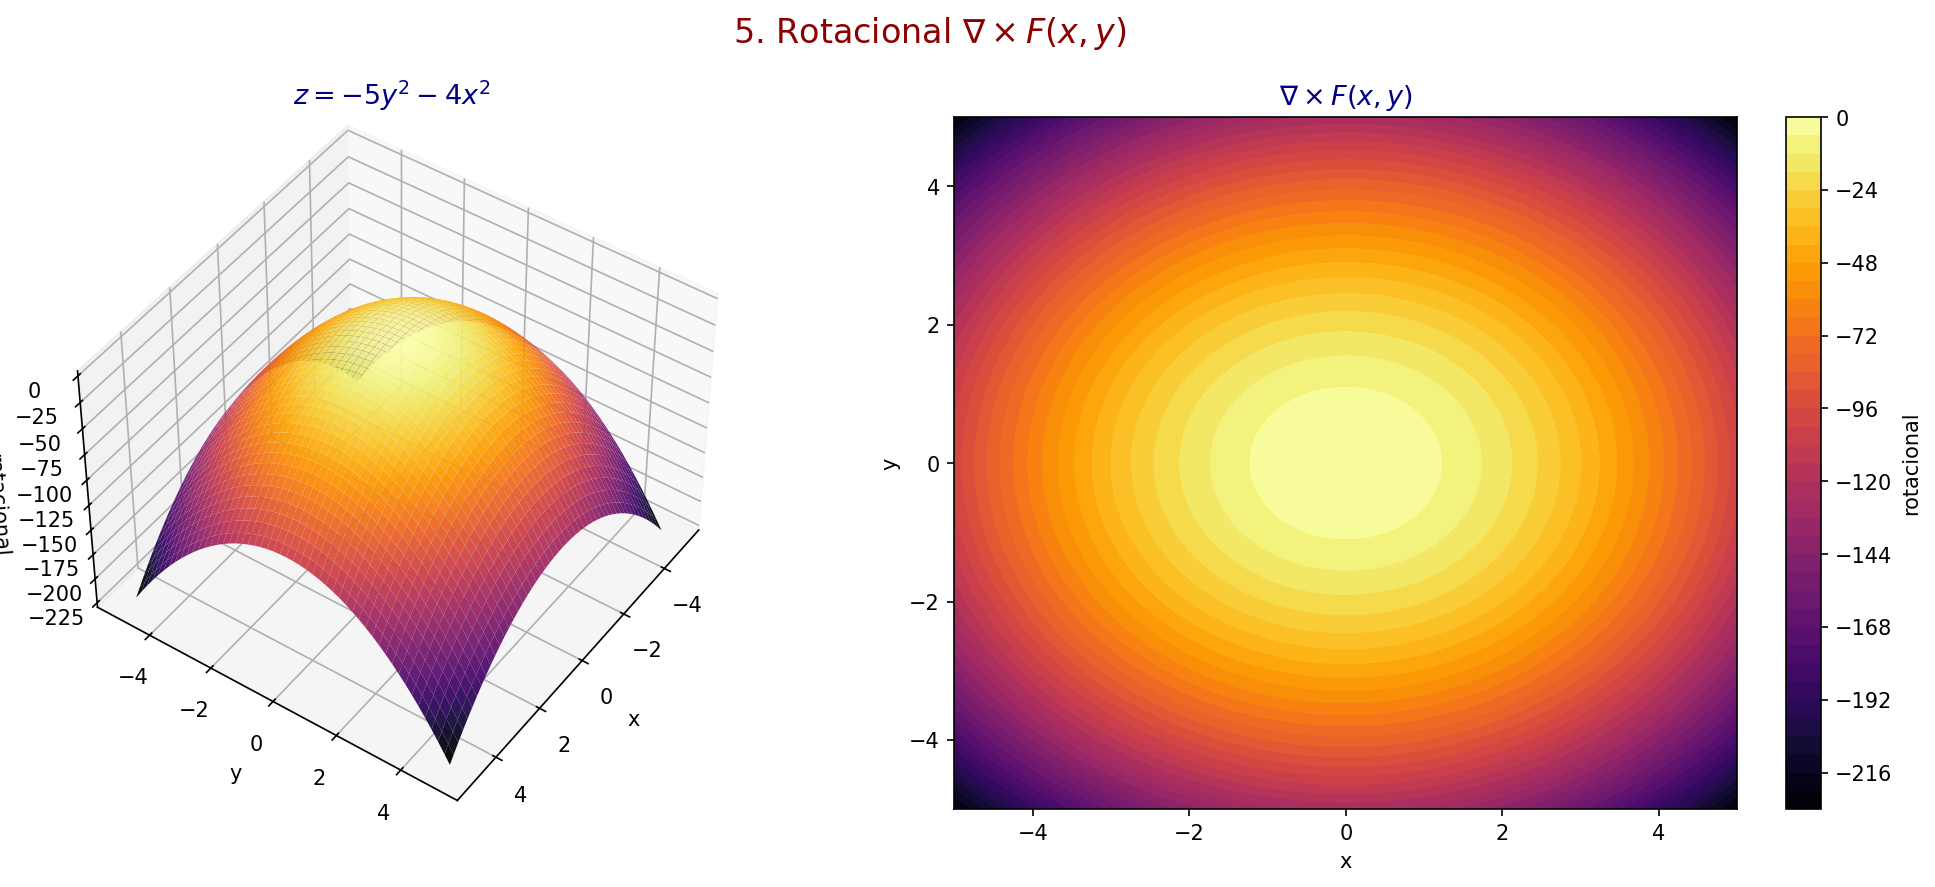
\includegraphics[width=\linewidth]{Images/Ejercicio_5_rotacional.png}
\caption{Gráficos del rotacional del campo vectorial $f(x,y) = \left(x^3+4x^2y, -5xy^2-y^3\right)$ visto como un campo 
escalar (izquierda) y como un mapa de calor (derecha).}
\end{figure}
\begin{lstlisting}[language=Python]
# dominio
x = np.linspace(-2,2,400)
y = np.linspace(-2,2,400)

X,Y = np.meshgrid(x,y)

# rotacional
Z = (
4*np.sin(X**2)*np.sin(Y)
-10*X*Y**3
+6*X**2*Y**2
)

# figura
fig = plt.figure(figsize=(14,6))

# --- superficie 3D ---
ax1 = fig.add_subplot(1,2,1, projection='3d')

surf = ax1.plot_surface(
    X,Y,Z,
    cmap='inferno',
    edgecolor='none',
    alpha=0.95
)

ax1.view_init(elev=60, azim=35)

ax1.set_title(
r"$z = 4\sin(x^2)\sin(y) -10xy^3 +6x^2y^2$",
fontsize=13,
color='navy'
)

ax1.set_xlabel("x")
ax1.set_ylabel("y")
ax1.set_zlabel("rotacional")

# --- mapa de temperatura ---
ax2 = fig.add_subplot(1,2,2)

cont = ax2.contourf(
    X,Y,Z,
    levels=40,
    cmap='inferno'
)

ax2.contour(
    X,Y,Z,
    levels=[0],
    colors='black',
    linewidths=1.2
)

ax2.set_title(
r"$\nabla \times F(x,y)$",
fontsize=13,
color='navy'
)

ax2.set_xlabel("x")
ax2.set_ylabel("y")

fig.colorbar(cont, ax=ax2, label="rotacional")

plt.suptitle(
r"6. Rotacional $\nabla \times F(x,y)$",
fontsize=16,
color='darkred'
)

plt.tight_layout()

fig.savefig(
'Imagenes/Ejercicio_6_rotacional.png',
dpi=150,
bbox_inches='tight'
)

plt.show()
\end{lstlisting}
\begin{figure}[H]
\centering
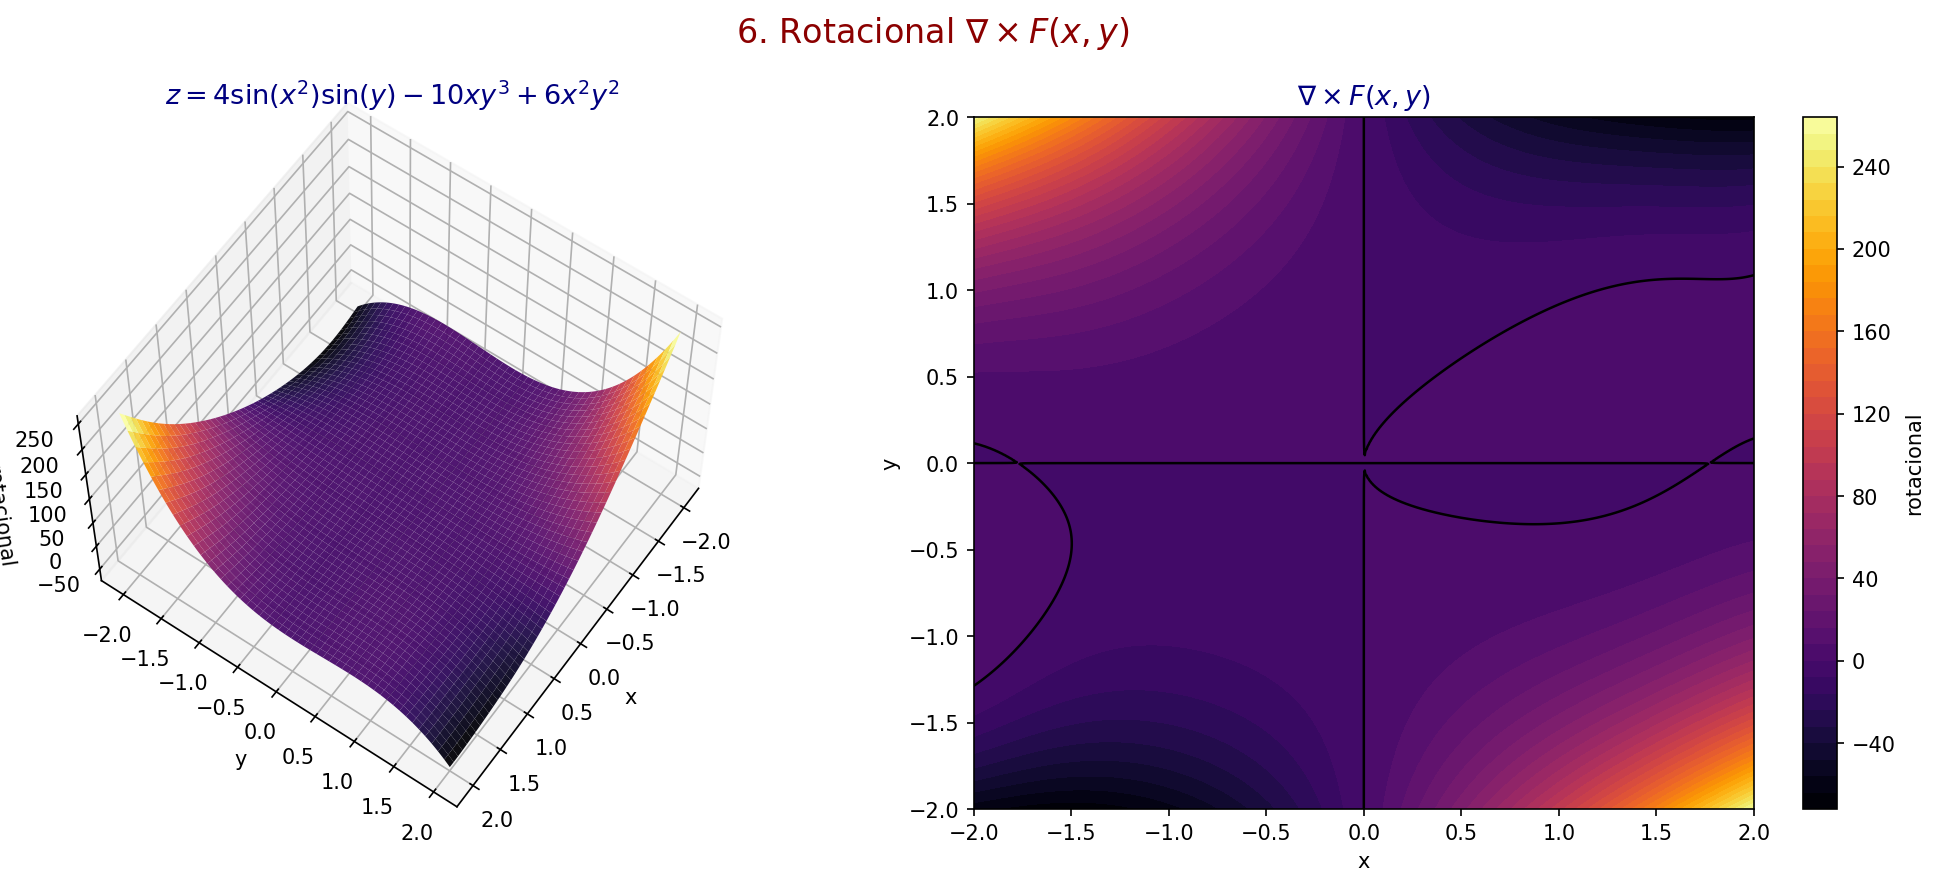
\includegraphics[width=\linewidth]{Images/Ejercicio_6_rotacional.png}
\caption{Gráficos del rotacional del campo vectorial $f(x,y) = \left(\cos(x^3) + 4\sin(x^2)\cos(y), 
-5x^2y^3+2x^3y^2\right)$ visto como un campo escalar (izquierda) y como un mapa de calor (derecha).}    
\end{figure}
